\thispagestyle{empty}
\vspace*{-16ex}
\centerline{\begin{tabular}{*3{c}}
	\parbox[t]{0.3\linewidth}{\begin{center}\textbf{Problem Chosen}\\ \Large \textcolor{red}{\Problem}\end{center}}
	& \parbox[t]{0.3\linewidth}{\begin{center}\textbf{2024\\ MCM/ICM\\ Summary Sheet}\end{center}}
	& \parbox[t]{0.3\linewidth}{\begin{center}\textbf{Team Control Number}\\ \Large \textcolor{red}{\Team}\end{center}}	\\
	\hline
\end{tabular}}

\begin{center}
	\Large \textbf{Shortest Path Algorithms:~Taxonomy and Advance in Research}
\end{center}

As for problem 1,  in order to accurately capture the effective information in the data 
set, we take a series of data processing methods... After that, we select potential influencing
factors and establish Analytic Hierarchy Process (AHP) model to make a preliminary analysis of the influencing
factors and calculate specific parameters for each factor. We find that the biggest factor is 
score difference. Apart from that ,whether scored in the last point, running distance, unforced error and fast win
will also positively or negatively influence the momentum to a comparatively large extent. The above conclusion is verified
in our later models.\\

In problem 2, we believe that momentum will affect the future scores of the match. So to answer the coach's question, 
we first perform autocorrelation test on momentum, and we find that it has strong first-oredr autocorrelation. Then we quantify 
the future scores and then determine the correlation of momentum the scores in the future, they are highly correlated.\\

Problem 3 is devided into 3 parts. To predict the swings in the match , we establish model based on Gated Recurrent Unit(GRU) algorithm.
We process data in problem 1 and add more features. We define the swings and use previous information to predict future.
Then compared to the result in problem 1, our accuracy is ....\\

To identify the most related factors, we use a novel argorithm called Permutation Feature Importance argorithm, 
it can determine the importance of features by calculating their prediction error after permutation. We find that ....\\

As for the ideas for specific atheletes, we use previous model on their matches to identify their feature importance.
We find that different atheletes have different features in their match.\\

Problem 4\\

Key words: AHP, correlation analysis, GRU, Permutation Feature Importance

Indroduction\\
Tennis more than any other sport, is a game of momentum. 
The absence of a clock to do the dirty work of finishing off an opponent, 
and a scoring system basedon units used, makes the flow of the match much more important than any 
lead that has been established.--Chuck Kriese\\

problem3

Using the above argorithm, we sort FI and normalize them, then we plot the figure:

\begin{figure}[H]
    \centering
    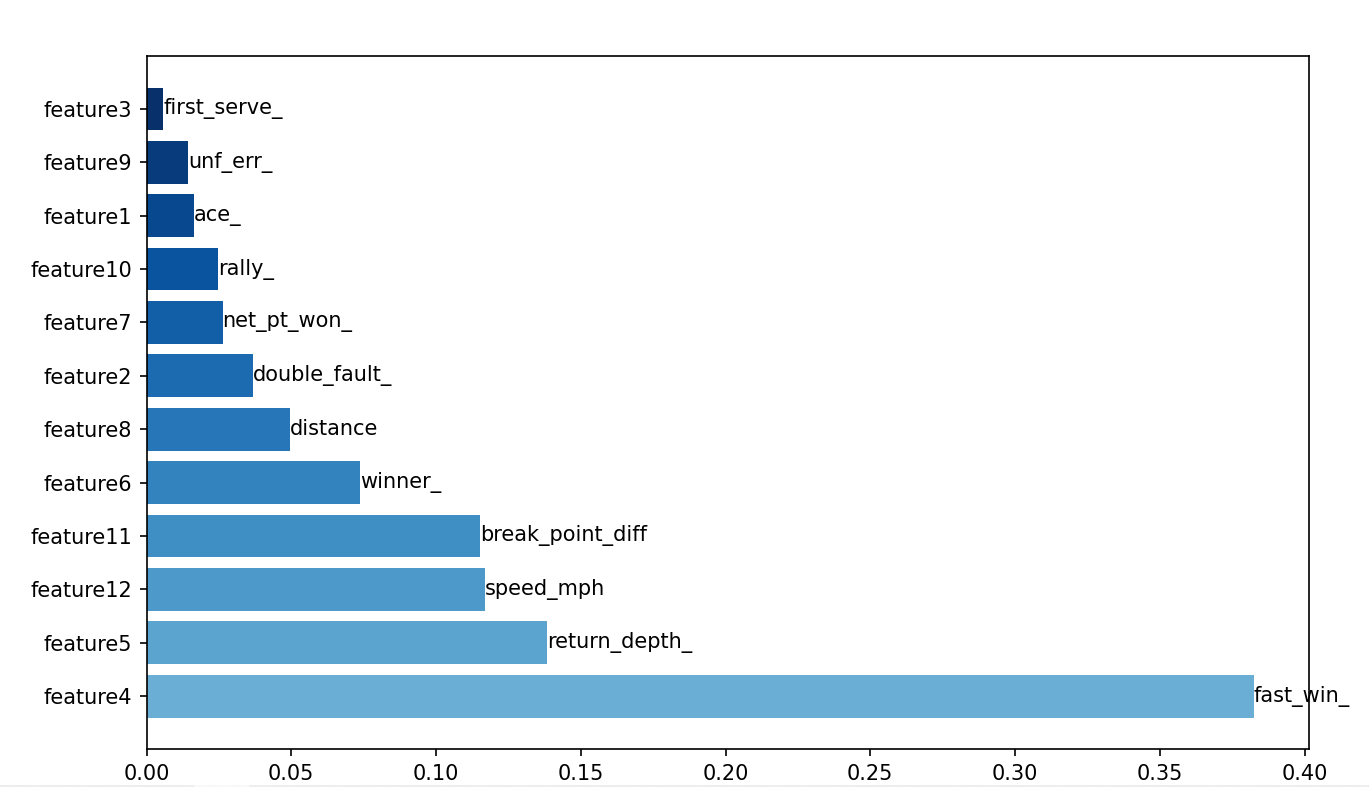
\includegraphics[scale=0.6]{mainmatter/imgs/8.png}
    \caption{feature importance}
\end{figure}

We can see that the most important feature is fast win(rally count < 3 and wins the point),
Because this time we only consider skill factors.this is related to our previous work,